\chapter{Time Series}

A \textbf{time series} is a collection of observations made sequentially in time, usually at constant time intervals. They can be constructed out of measurements of many different phenomenons, such as annual rainfall levels, earthquakes, fMRI data, quarterly earnings, audio/video data, and so on. Time series can analyzed through clustering, classification, motif discovery, rule discovery, forecasting, and trend/seasonality analysis. The key issues that arise when working with time series are:
\begin{itemize}
    \item \textbf{The amount of data to work with can be incredibly large}: for datasets with several different sources and short intervals of time between measurements, the size can be very high.

    \item \textbf{Similarity is not easy to estimate}: since series are complex objects with several values each, defining how two series can be considered similar is not as easy as it can be for numerical data.

    \item \textbf{Different data formats}: different series in the same dataset may be represented using a different scale or format; e.g., atmospheric temperatures recorded in both $^{\circ}C$ and $^{\circ}F$.

    \item \textbf{Different sampling rates}: while usually it is assumed that series are recorded all with the same rate, in many real life cases this may not be true. Different series may have different lengths and different time intervals.

    \item \textbf{Noise, missing values, and other defects}: as with other types of data, time series can also present noisy information or missing values.
\end{itemize}
The following sections will explain how some of these issues can be dealt with.

\section{Similarity Between Time Series}

\subsection{Structural-based Similarities}

Especially when analyzing long time series, similarity is calculated on a structural level. This means that global features are extracted from the time series, creating a feature vector, and measuring similarity looking at those features. Some examples are the mean and variance, maximum/minimum, skewness, mean and variance of the $1^{st}$ derivative, and so on.

A measure used to calculate structural dissimilarity is \textbf{compression based dissimilarity}, which is calculated as:
\begin{equation*}
    d(x,y) = CDM(x,y) = \dfrac{C(x,y)}{C(x) + C(y)} \,,
\end{equation*}
where $C$ is a compression algorithm. The numerator is the compression of the concatenation of the two series, while the denominator is the sum of the compressions of the series done singularly: the Compression Dissimilarity Measure equal to 1 if the two series are unrelated, otherwise it is less than one. The smaller its value, the closer the series are to each other. CDM is never zero.

\subsection{Shape-based Similarities}

Shape-based similarities can be calculated using distance measures. Recall that distances have the following properties:
\begin{align*}
    &d(a,b) \geq 0, d(a,b) = 0 \iff a = b \ (Positivity) \\
    &d(a,b) = d(b,a) \ (Symmetry) \\
    &d(a,c) \leq d(a,b) + d(b,c)
\end{align*}
One way to calculate shape-based dissimilarity is using Euclidean distance. Given two time series (with the same exact number of points/measurements), the Euclidean distance is calculated as if the series were points in an Euclidean space. However, this distance is very sensitive to distortions in the data, which should be removed in a preprocessing phase.

The most common distortions are:
\begin{itemize}
    \item \textbf{Offset translation}: the series have different offsets on the y axis. Calculating the distance without addressing this problem would return a value that is drastically larger than the actual shape distance. This can be corrected by subtracting each series with its own mean value.
    \begin{figure}[h]
        \centering
        \begin{minipage}{0.40\textwidth}
         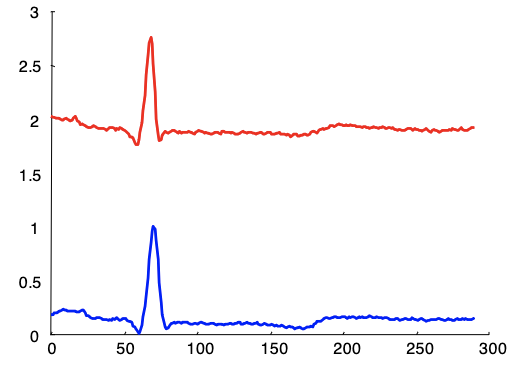
\includegraphics[width=1.0\linewidth]{img/offset_trans_1.png}
        \end{minipage}
        \hfill
        \begin{minipage}{0.40\textwidth}
            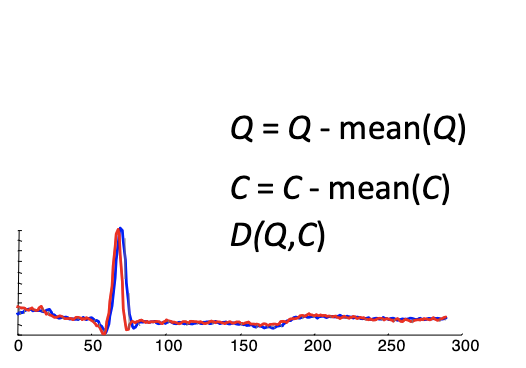
\includegraphics[width=1.0\linewidth]{img/offset_trans_2.png}
        \end{minipage}
        \label{fig:offset-trans}
        \caption{Offset translation transformation.}
    \end{figure}

    \item \textbf{Amplitude scaling}: the series have the same shape, but are scaled differently on the y axis. This is corrected by applying Z-score normalization to the values of the series (subtracting the mean and dividing by the standard deviation).
    \begin{figure}[h]
        \centering
        \begin{minipage}{0.40\textwidth}
            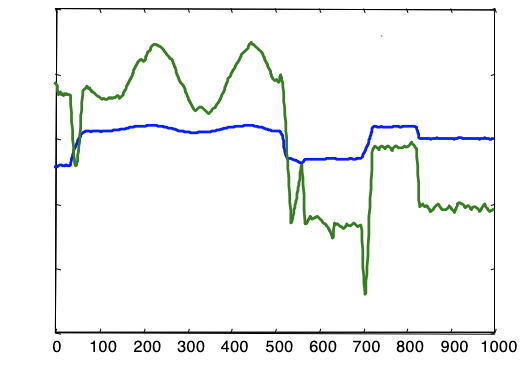
\includegraphics[width=1.0\linewidth]{img/ampli_scaling_1.png}
        \end{minipage}
        \hfill
        \begin{minipage}{0.40\textwidth}
            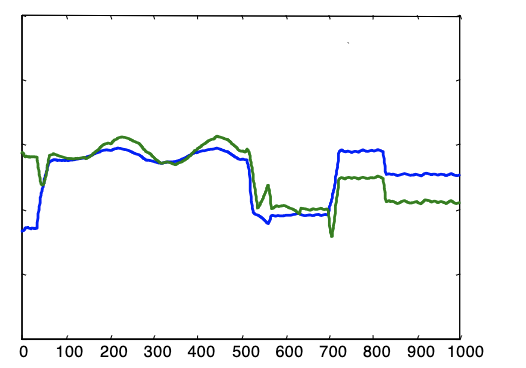
\includegraphics[width=1.0\linewidth]{img/ampli_scaling_2.png}
        \end{minipage}
        \caption{Amplitude scaling transformation.}
        \label{fig:ampli-scaling}
    \end{figure}

    \item \textbf{Linear trend}: series can follow upwards or downwards linear trends, which means that as they progress they increase or decrease in level. This can be corrected by finding the best fitting line to a time series, and subtracting it from the time series itself.
    \begin{figure}[h]
        \centering
        \begin{minipage}{0.40\textwidth}
            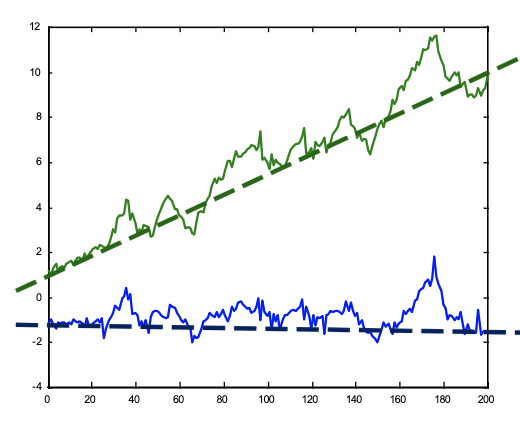
\includegraphics[width=1\linewidth]{img/lin_trend_1.png}
        \end{minipage}
        \hfill
        \begin{minipage}{0.40\textwidth}
            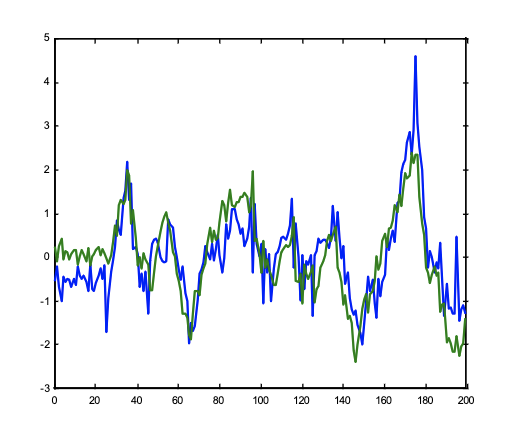
\includegraphics[width=1\linewidth]{img/lin_trend_2.png}
        \end{minipage}
        \caption{Linear trend transformation.}
        \label{fig:lin-trend}
    \end{figure}

    \item \textbf{Noise}: noise is the presence of random error in the series. To remove noise, each data point can be replaced with the average value of its neighbors.
    \begin{figure}[h]
        \centering
        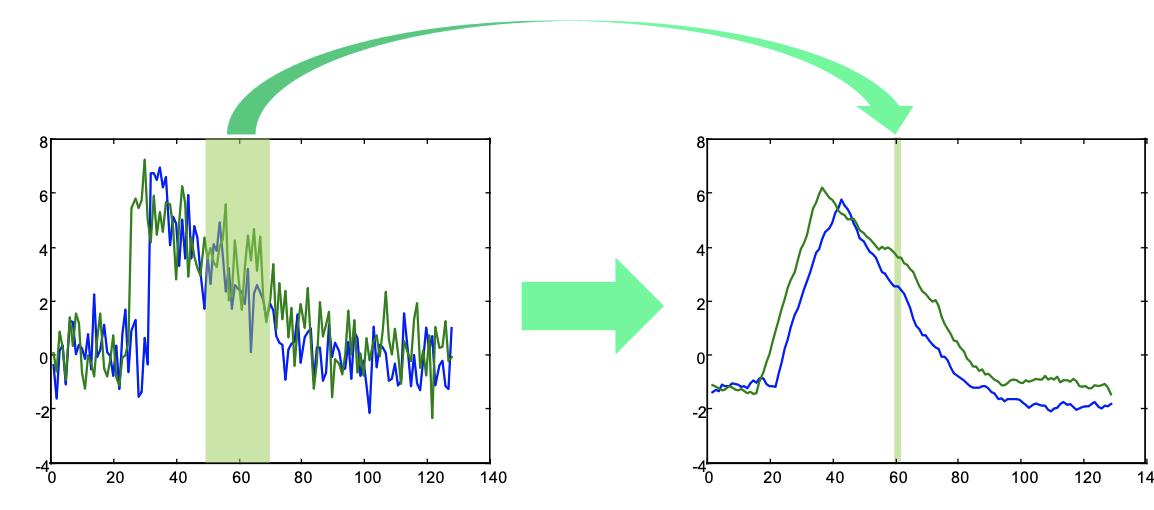
\includegraphics[width=0.80\linewidth]{img/noise_trans.png}
        \caption{Noise transformation.}
        \label{fig:noise-trans}
    \end{figure} \\
    Noise can be removed by a \textbf{moving average} (\textbf{MA}): given a window of length $w$ and a time series $t$, the MA is applied as:
    \begin{equation*}
        t_i = \dfrac{1}{w} \sum_{j=i-w/2}^{w/2} t_j \ i = 1, \dots , n
    \end{equation*}
\end{itemize}

\subsubsection{Dynamic Time Warping}

It's often the case that two time series have approximately the same shape, but they do not line up on the x axis. The euclidean distance calculated between such series would be high, despite them being similar: this is because it considers a fixed time axis for both series. In order to find the similarity between them, the time axis must be ``warped'' for one or both time series to align them correctly.

In practice, DTW is calculated in three steps. First, given the series $Q$ and $C$, a matrix of size $|Q| \times |C|$ is constructed, and each cell of index $i,j$ contains the distance between the $i^{th}$ component of $Q$ and the $j^{th}$ component of $C$. The diagonal of this matrix corresponds to the comparison done by the Euclidean distance. Every possible warping between two time series corresponds to a path from the bottom left corner $(0,0)$ and the top right corner $(0,|C|)$ of the matrix. The DTW will be the best path, i.e., the one that yields the lowest sum of costs. The best path is found recursively, using the following formula:
\begin{equation*}
    \gamma(i,j) = d(q_i,c_j) + \min\{\gamma(i-1, j-1), \gamma(i-1, j), \gamma(i, j-1)\}
\end{equation*}

The dynamic programming approach to the problem starts by calculating the distance matrix for the two series; then, the matrix of cumulative costs for each path; finally, the path with the best alignment is found, connecting the cells with the lowest cost.
\begin{figure}[h]
    \centering
    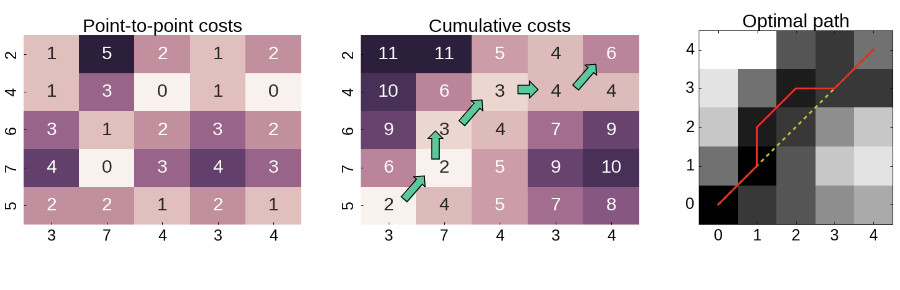
\includegraphics[width=1.0\linewidth]{img/dtw.png}
    \caption{How Dynamic Time Warping is calculated.}
    \label{fig:dtw}
\end{figure}